\section{Case Study: Power Saving of Dark Mode}
\label{sec:casedark}

% \subsection{Rise of dark mode}
% Platform dark mode - Android P
% App dark mode -- how many apps in Google Play support dark mode?

\forjnl{
  The per-frame OLED power profiler can be used by developers to gain
insight into and optimize the power draw of the app activity UI
design, and Battery+ can be used by phone users to understand and manage
phone display energy drain, for example, from different app and
display configurations.
}

In this section, we present a case study of
how the tools help developers and phone users to quantify and manage
the power saving of the dark mode for a set of popular
Google apps
%  and Android system apps 
(each with 1B+ downloads).
% These apps are ubiquitous and used by a large number of users.



\subsection{Power Saving for Typical App Usage Scenarios}
\label{subsec:mainresults}

We first show how Battery+ helps phone users to easily learn the
impact of dark mode on OLED and the whole phone battery drain.

\begin{table*}[tb]
\caption{List of apps and test scenarios used in our dark mode energy saving study.}
\label{tab:app_usage_scenarios}
\vspace{-0.1in}
\begin{minipage}{\textwidth}
\centering
{\footnotesize
      \begin{tabular}{|l|c|c|m{.5\textwidth}|}
\hline
\makecell{Apps\\(version)} & \makecell{Test\\scenario} & \makecell{Test\\duration\\} & \makecell{Actions} \\
\hline
Calculator & Various calculations & 60 s & Compute the first 20 Fibonacci numbers. \\
\hline
Google Phone & \makecell{Create a new contact and\\ dial a number} & 60 s & Create 2 new contacts. Check the call history and dial a number. \\
\hline
Google Calender & \makecell{Check, create and\\ delete appointment} & 60 s & Create a new appointment. Delete the appointment. Check for appointment in the Day, Week and Month views.  \\
\hline
Google Maps & Search and navigate & 60 s & Search for nearby gas station and start navigation. \\
\hline
Google News & Reading News & 60 s & Open a section and scroll in it. \\
\hline
YouTube & \makecell{Search and\\ watch a video} & 60 s & Open the app. Search keywords in the serach. Pick the first video and watch for 10 secs. Leave the video. Repeat 2 times.\\
\hline
\end{tabular}
    }
\end{minipage}
\end{table*}
\paragraph{Methodology.}
Table~\ref{tab:app_usage_scenarios} lists the 6 popular Google apps 
in our experiment which all have recently introduced support for dark mode.
We run each app under a
typical user interaction (listed in Table~\ref{tab:app_usage_scenarios})
that lasts about 60 seconds.  To ensure the identical
user interactions are performed under both light mode and dark mode, we
use UIAutomator 2 and Appium~\cite{appium} to drive precoded user
interactions for the apps.
% The screen was recorded using Android screenrecord command.
% The screen brightness was set to 100\%.
%   The average current consumed by the phone
%   {is measured using built-in power sensors and forms the basis for the ground truth
%   on the total phone power draw.
%   }

\begin{figure*}[tb]
	\begin{subfigure}[]{0.32\textwidth}
		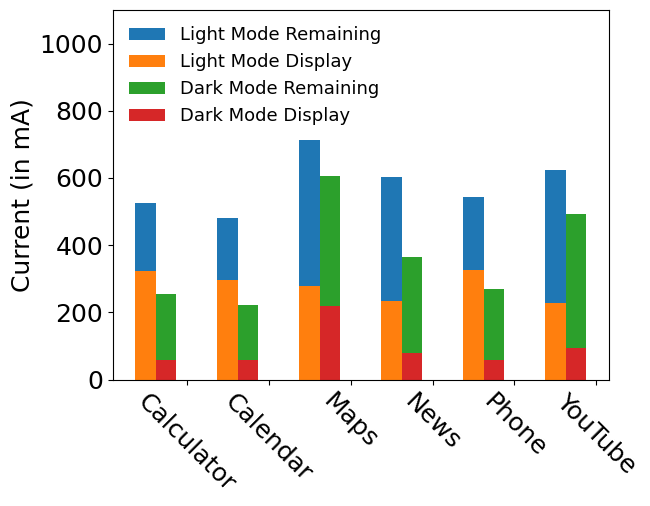
\includegraphics[width=\textwidth]{figure/002_Pixel2_case_study.png}
        \vspace{-0.2in}
		\caption{Pixel 2}
	\end{subfigure}
	\begin{subfigure}[]{0.32\textwidth}
		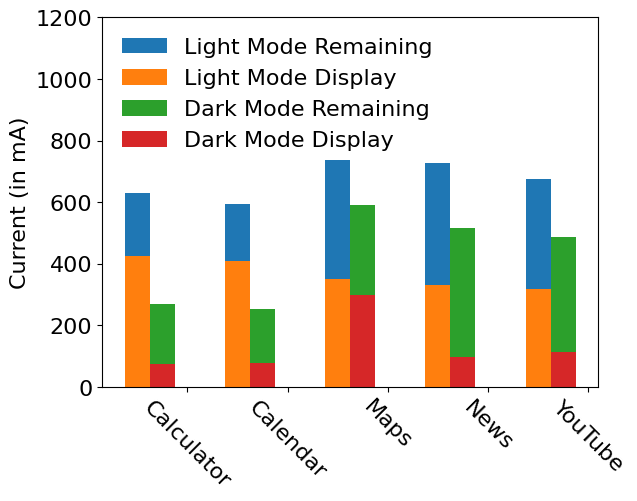
\includegraphics[width=\textwidth]{figure/003_MotoZ3_case_study.png}
        \vspace{-0.2in}
		\caption{Moto Z3}
	\end{subfigure}
	\begin{subfigure}[]{0.32\textwidth}
		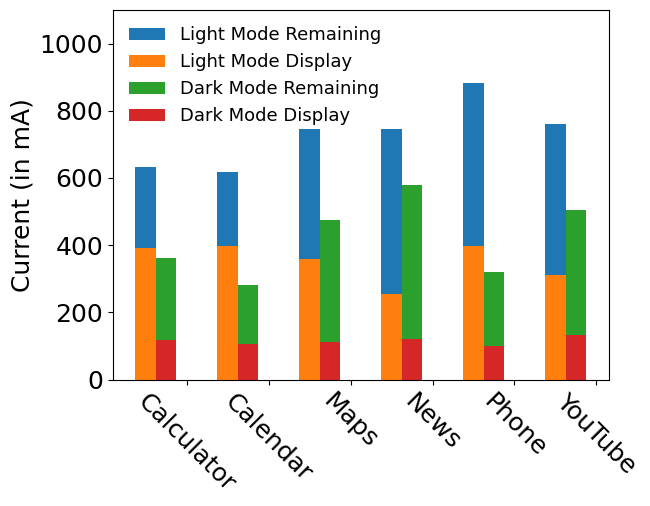
\includegraphics[width=\textwidth]{figure/004_Pixel4_case_study.png}
        \vspace{-0.2in}
		\caption{Pixel 4}
	\end{subfigure}
        \vspace{-0.15in}
	\caption{Total phone and OLED power draw under light mode and dark mode
 on the three phones.}
        \vspace{-0.10in}
	\label{fig:apps_expriment}
\end{figure*}

\paragraph{Impact of dark mode.}
Figure~\ref{fig:apps_expriment} shows the total phone power draw and
the OLED display power draw portion reported by Battery+
running on the 3 phones for the 6 Google apps at 100\% brightness.
We make the following observations.
%
(1) In light mode,
the OLED display draws a significant portion of the total phone power,
ranging between 
37\%-62\%, 45\%-69\%, and 34\%-64\% \comment{check these numbers??? DONE}
across the 6 Android apps on Pixel 2, Moto Z3 and Pixel 4, respectively.
%   across the 3 phones, for the same apps ,OLED average power draw is
%   187 mA,250 mA,233 mA which is (18\% - 61\%),(33\% - 84\%),(21\% -
%   64\%) of the total phone power draw for Pixel 2 , Moto Z3 and Pixel 4
%   respectively.
%
%(2) The major power difference comes from non-OLED components --
%the average non-OLED component power draw is reduced
%from 606 mA on Nexus 6 to 223 mA and 165 mA on the newer Pixel 2 and Moto Z3,
%from improved system components and SoC integration.
%In contrast, the OLED display power draw stays similar across the 3 phones --
%the average across the apps actually increases by 27\% from Nexus 6 to Moto Z3.
%
(2) Switching from light to dark mode significantly
reduces the OLED power draw across all apps, by
21\%-82\% (average 65\%), 14\%-82\% (average 62\%), and 52\%-74\%  (average 66\%)
across the 6 apps on the 3 phones, respectively. 
(3) This large OLED power reduction translates into
major reduction in the total phone power,
ranging between 15\%-53\% (average 38\%), 19\%-57\% (average 38\%), and 22\%-63\%  (average 42\%)
across the apps on the 3 phones.
Interestingly,
% In other words, 
%though dark mode leads to higher OLED power savings on the older Nexus 6 phone, 
the overall phone power saving comes out to
be similar across the 3 phones.
%, because the non-OLED component power
%draw was also higher on Nexus 6.
%
%   (5) \comment{
%     The apps can be grouped into three categories based on
%   the level of power reduction in dark mode:
%   Google Calender,Phone ,Calculator \& News which experience higher reduction,
%   Google Maps and News which experiences moderate reduction,
%   and Youtube which experiences a low reduction.
%   }
%  (6)YouTube display
%  power consumption is somehow comparable to Google text heavy apps i.e
%  Google Calender,Phone ,Calculator.
While we used UIanimator and Appium to measure the precise
power reduction from switching from light to dark mode for the same apps,
a phone user can easily use Battery+ to get the approximate power reduction value
by manually repeating the same app run, \eg for 1 minute.


\paragraph{Impact of screen brightness.}
\if 0
Applying the correlation between screen brightness level and the OLED
power adjustment that we derived in
\S\ref{subsec:brightness}, we can directly derive the OLED power draw
for displaying any frame under any different brightness level from
that measured under brightness level 100\%.
We apply this technique to the results in
\fi
As discussed in \S\ref{subsec:brightness}, changing the brightness level
  affects the OLED power draw in complicated ways on Pixel 2 , Moto Z3 and Pixel 4.
%   \comment{We therefore regenerated the P-LMLR model for 30\% and 50\% brightness level
%   on all 3 phones phones} and
  % Figure~\ref{fig:apps_expriment}
  Table~\ref{fig:powerreductionbrightness}
  shows the OLED/whole phone power saving under brightness levels 30\%, 50\%
  and 100\%.
We make two observations.
(1) As expected, the lower the brightness level, the less power saving from switching
to  dark mode. In particular, 
the average OLED power saving across the apps on the 3 phones
in switching to dark mode is reduced
from 65\%, 62\%, and 66\% under 100\% brightness level
to 24\%, 25\%, and 19\% under 50\% brightness level
and 12\%, 14\%, and 9\% under 30\% brightness level,
and the average phone power saving across the apps on the 3 phones
is significantly diminished
from 38\%, 38\%, and 42\% under 100\% brightness level
to 7\%, 5\%, and 10\% under 50\% brightness level
and 4\%, 5\%, and 6\% under 30\% brightness level, respectively.
(2) The OLED power reductions under dark mode for Google Maps, News and YouTube 
are lower than those for the other apps. This is because these 3 apps
display static (images) or dynamic (videos) embedded objects % during app run
which are not affected by dark mode.
We note that the small negative reduction in total phone power for some apps under 30\% brightness
happens because the display power at this brightness level is already a small portion
of the total power and slight perturbation in the experiment causes the total power to go up or down.


\begin{table*}[htb]
\caption{Power reduction when switching from light to dark mode at
  different screen brightness levels.
  X/Y: display power reduction / total phone power reduction. %\footnotemark
  The Phone app is not supported on Moto Z3.}
\vspace{-0.1in}
\centering
{ \footnotesize
\begin{tabular}{ | l | c | c | c | c | c | c | c | c | c |}
  \hline
  & \multicolumn{9}{ c |}{Brightness Level} \\
	\cline{2-10}
	& \multicolumn{3}{ c |}{Pixel 2} & \multicolumn{3}{ c |}{Moto Z3} & \multicolumn{3}{ c |}{Pixel 4} \\
	\cline{2-10}
	App
	& 30\%  & 50\%  & 100\% 
        & 30\%  & 50\%  & 100\% 
        & 30\%  & 50\%  & 100\%  \\
	\hline
	Calculator    
	    &  17\%/   7\% &  33\%/  11\% &  81\%/  51\%         
        &  20\%/   8\% &  35\%/  13\% &  82\%/  57\%
        &  10\%/   4\% &  22\%/   8\% &  69\%/  42\% \\
	Google Phone            
	    &  17\%/   5\% &  34\%/   9\% &  82\%/  50\%
        &    -    &    -    &   - 
        &  11\%/   9\% &  24\%/  15\% &  74\%/  63\% \\
	Google Calendar
        &  16\%/   7\% &  31\%/  15\% &  79\%/  53\%
        &  19\%/   7\% &  34\%/  10\% &  80\%/  57\%
        &  11\%/   3\% &  23\%/  13\% &  73\%/  54\% \\
	Google Maps
        &   4\%/   0\% &   4\%/  -3\% &  21\%/  15\% 
        &    6\%/   8\% &  12\%/ -12\% &  14\%/  19\%
        &    9\%/   9\% &  20\%/  15\% &  69\%/  36\% \\
	Google News
        &  10\%/   4\% &  21\%/   8\% &  66\%/  39\%
        &  12\%/   2\% &  24\%/  11\% &  70\%/  28\%
        &   5\%/   3\% &  12\%/   0\% &  52\%/  22\% \\
	YouTube         
	    &   9\%/   3\% &  19\%/   1\% &  59\%/  20\%
        &  13\%/   3\% &  22\%/   7\% &  63\%/  28\%
        &   6\%/   6\% &  14\%/  10\% &  56\%/  33\% \\
        \hline
	Average
	    &  12\%/   4\% &  24\%/   7\% &  65\%/  38\%
        &  14\%/   5\% &  25\%/   5\% &  62\%/  38\%
        &   9\%/   6\% &  19\%/  10\% &  66\%/  42\% \\
	\hline
\end{tabular}
}
\label{fig:powerreductionbrightness}
\end{table*}
% \footnotetext{For some apps for 30\% brightness we has negative reduction in total power.
% This is due to the display contribution at this brightness is very less
% as compared to total power. The difference between the dark mode and light mode
% can be as less as 10 mA.
% The slight perturbation in experiment gets reflected in the total power
% consumption.}

% \begin{table*}
% \caption{Apps, their statistics, and test scenarios.}
% \label{tab:scenarios}
% \vspace{-0.1in}
% \begin{minipage}{\textwidth}
% \centering
%     {\small
%       \begin{tabular}{l|c|c|m{.5\textwidth}}
% \hline
% \makecell{Apps\\(version, size, installs)} & \makecell{Test\\scenario} & \makecell{Test\\duration\\} & \makecell{Actions} \\
% \hline
% \multirow{2}{*}[.7em]{\makecell[l]{Messenger\\(214.0.0.20.111, 116MB, 1B+)\\Messenger Lite\\(57.0.0.19.208, 21MB, 100M+)}}
% & \makecell{Send\\text}
% & 150s
% & Click the text field. Type a 20 character random string. Send. The message is delivered to the peer, but not seen\footnote{A message can have one of three status in Messenger and Messenger Lite depending on the peer: sent, delivered or seen. The status will affect the traffic.}. Repeat 10 times. \\
% \cline{2-4}
% & \makecell{Send\\stickers}
% & 150s
% & Send the smiling face sticker. The message is delivered to the peer, but not seen. Repeat 30 times. \\
% \hline
% \makecell[l]{Twitter\\(7.97.1-release.59, 57MB, 500M+)\\Twitter Lite (2.1.2--28, 4MB, 10M+)}
% & Scroll
% & 150s
% & Click the profile picture in the first tweet. Then scroll 30 times. \\
% \hline
% \makecell[l]{Opera\\(52.2.2517.139816, 90MB, 100M+)\\Opera Mini\\(42.0.2254.139276, 28MB, 100M+)}
% & \makecell{Google\\search}
% & 150s
% & Click the omnibar. Enter the keywords. Click the search button. Repeat with 5 different trending keywords. \\
% \hline
% \makecell[l]{Google (9.91.6.21.arm, 60MB, 5B+)\\Google Go\\(2.6.250469770.release, 21MB, 50M+)}
% & Search
% & 200s
% & Click the search bar. Enter the keywords. Click the search button. Go back to app home screen. Repeat with 5 different trending keywords. \\
% \hline
% \makecell[l]{Google Maps (10.17.2, 91MB, 5B+)\\Google Maps Go (98, 311KB, 50M+)}
% & Restaurants
% & 150s
% & Search for a list of nearby restaurants. For the first 5 results, click on each one to show their detailed pages. \\
% \hline
% \end{tabular}
%     }
% \end{minipage}
% \end{table*}


% \subsection{Ground Truth}
% \label{subsec:goundesults}

% To capture the accuracy of the P-LMLR and Battery+, we created an
% Android App with ExoPlayer video player library.  During the case
% study we capture the screen using {\tt screenrecord}.  For each app
% and brightness level we ran the video four times 1) with
% corresponding brightness level, 2) dark screen (brightness set to
% zero), 3) dark screen with {\tt screenrecord} running and 4) dark
% screen with Battery+ running.  We found the average power consumed
% by Battery+ by subtract case 2 from case 4, the average OLED power
% by subtracting case 2 from case 1, and power consumed by
% screenrecord by subtracting case 2 from case 3.  % The results are
% presented in Table~\ref{tab:displaygroundtruth}.  The average
% current consumed by Battery+ is 14.17 mA, 87.83 mA and 22.83 mA for
% the 3 phones, respectively.  We then found the error between the
% estimated display power and the ground truth display power.  The
% error is tabulated in Table~\ref{tab:batt_error}.  We observed that
% the estimation error is higher at lower brightness and for dark mode
% due the fact the display power is lower.  The mean prediction error
% in estimating the error is 12.17 \%, 6.03 \% and 9.50\% for the 3
% phones, respectively.

% \begin{table}[tp]
% \begin{center}
% \centering
% \caption{Mean prediction display error for the 6 apps.}
% \vspace{-0.1in}
% \footnotesize
% \begin{tabular*}{\columnwidth}{@{\extracolsep{\fill}}|l|c|c|c|c|}
% 	\hline
% 	       \multirow{2}{*}{Phone} & \multirow{2}{*}{Mode} & \multicolumn{3}{c|}{Brightness} \\
% 	\cline{3-5}
% 	        &   & 30\% & 50\% & 100\% \\
% 	\hline
% 	\multirow{2}{*}{Pixel 2} &       Dark & 12.3\% & 15.0\% & 14.4\% \\
% 	                         &      Light & 14.3\% & 12.9\% &  4.1\% \\
% 	\hline
% 	\multirow{2}{*}{Moto Z3} &       Dark &  4.4\% &  5.8\% & 14.4\% \\
% 	                         &      Light &  4.1\% &  3.5\% &  4.0\% \\
% 	\hline
%     \multirow{2}{*}{Pixel 4} &       Dark &  2.8\% &  2.5\% &  8.5\% \\
%                              &      Light & 35.4\% &  3.8\% &  4.0\% \\
% 	\hline
% \end{tabular*}
% \label{tab:batt_error}
% \end{center}
% \vspace{-0.15in}
% \end{table}

% \begin{table*}[tp]
% \caption{ The ground truth current in mA for for the 6 apps in the case study. (Display Current/Battery+ Current/Screenrecord Current)
%   The Phone app is not supported on Moto Z3.}
% \vspace{-0.1in}
% \centering
% { \footnotesize
% \begin{tabular}{ | l | c | c | c | c | c | c | c | c | c | c |}
%   \hline
%     & & \multicolumn{9}{ c |}{Brightness Level} \\
% 	\cline{3-11}
% 	& & \multicolumn{3}{ c |}{Pixel 2} & \multicolumn{3}{ c |}{Moto Z3} & \multicolumn{3}{ c |}{Pixel 4} \\
% 	\cline{3-11}
% 	App & Mode
% 	& 30\%  & 50\%  & 100\% 
%         & 30\%  & 50\%  & 100\% 
%         & 30\%  & 50\%  & 100\%  \\
% 	\hline
% 	Calculator
% 	    & Dark
% 	    &  49/  4/ 60 &  39/ 10/ 52 &  64/  5/ 55         
%         &  62/ 57/ 45 &  60/ 57/ 45 &  83/ 52/ 47
%         &  87/ 16/ 62 &  79/ 10/ 64 & 109/ 13/ 64 \\
%         & Light
% 	    &  66/ 27/ 74 &  58/ -5/ 49 & 329/ 23/ 65         
%         &  76/ 55/ 49 &  96/ 58/ 48 & 430/ 54/ 45
%         &  94/ 18/ 70 & 109/ 13/ 64 & 397/ 11/ 53 \\
%         \hline
% 	Google Phone
% 	    & Dark
% 	    &  49/ 17/ 65 &  54/ 14/ 65 &  56/  6/ 62
%         &    -    &    -    &   - 
%         &  78/ 10/ 45 &  80/ 14/ 47 &  91/ 16/ 53 \\
%         & Light
% 	    &  64/ 20/ 58 &  60/  0/ 48 & 331/ 18/ 63         
%         &    -    &    -    &   -
%         &  86/ 11/ 61 & 108/ 20/ 66 & 428/ 20/ 73 \\
%         \hline
% 	Google Calendar
% 	    & Dark
%         &  57/ 20/ 56 &  58/ 17/ 64 &  76/ 26/ 66
%         &  59/ 50/ 39 &  64/ 54/ 43 &  87/ 43/ 35
%         &  82/ 15/ 43 &  81/ 11/ 44 & 105/ 14/ 60 \\
%         & Light
% 	    &  52/ -3/ 49 &  80/  4/ 42 & 317/ 15/ 47         
%         &  77/ 48/ 41 &  95/ 43/ 41 & 426/ 46/ 38
%         &  100/ 17/ 56 & 108/ 10/ 44 & 427/ 14/ 47 \\
%         \hline
% 	Google Maps
% 	    & Dark
%         &  45/ 16/ 80 &  57/  5/ 69 & 156/ 16/ 81 
%         &  65/ 78/ 66 &  77/ 86/ 69 & 218/ 74/ 65
%         &  83/ 14/ 67 &  82/ 19/ 68 & 105/ 12/ 71 \\
%         & Light
% 	    &  65/  9/ 80 &  57/  2/ 57 & 247/ 24/ 65         
%         &  73/ 80/ 71 &  86/ 58/ 49 & 345/ 79/ 68
%         &  93/ 17/ 85 &  98/ 13/ 68 & 350/ 18/ 67 \\
%         \hline
% 	Google News
% 	    & Dark
%         &  43/ 11/ 88 &  41/  2/ 94 &  84/ 18/ 98
%         &  62/151/154 &  67/133/125 & 107/121/127
%         &  82/ 56/189 &  90/ 57/189 & 106/ 49/171 \\
%         & Light
% 	    &  48/  3/ 81 &  64/ 23/102 & 239/ 35/186         
%         &  70/152/153 &  84/147/148 & 361/143/135
%         &  30/ 65/184 & 102/ 47/185 & 268/ 53/191 \\
%         \hline
% 	YouTube
% 	    & Dark
% 	    &  55/ 20/110 &  57/ 22/106 & 107/ 35/119
%         &  67/119/107 &  70/117/107 & 126/119/103
%         &  81/ 21/107 &  85/ 23/118 & 121/ 15/115 \\
%         & Light
% 	    &  66/ 14/106 &  66/ 20/115 & 229/  8/103         
%         &  73/116/105 &  85/124/112 & 339/120/109
%         &  91/ 26/129 & 102/ 32/120 & 314/ 35/137 \\
%         \hline
% 	Average
% 	    & Dark
% 	    &  50/ 15/ 76 &  51/ 12/ 75 &  90/ 18/ 80
%         &  63/ 91/ 82 &  68/ 90/ 78 & 124/ 82/ 75
%         &  82/ 22/ 85 &  83/ 22/ 88 & 106/ 20/ 89 \\
%         & Light
% 	    &  60/ 12/ 75 &  64/  7/ 69 & 282/ 21/ 88         
%         &  74/ 90/ 84 &  89/ 86/ 80 & 380/ 88/ 79
%         &  82/ 25/ 98 & 105/ 23/ 91 & 364/ 25/ 95 \\
% 	\hline
% \end{tabular}
% }
% \label{tab:displaygroundtruth}
% \end{table*}






\begin{figure}[tb]
	\begin{subfigure}[]{\columnwidth}
		\centering
		% \includegraphics[width=0.58\columnwidth]{./figure/609_news_light.pdf}\quad
		% \frame{\includegraphics[width=0.27\columnwidth]{./figure/659_news_light.png}}
		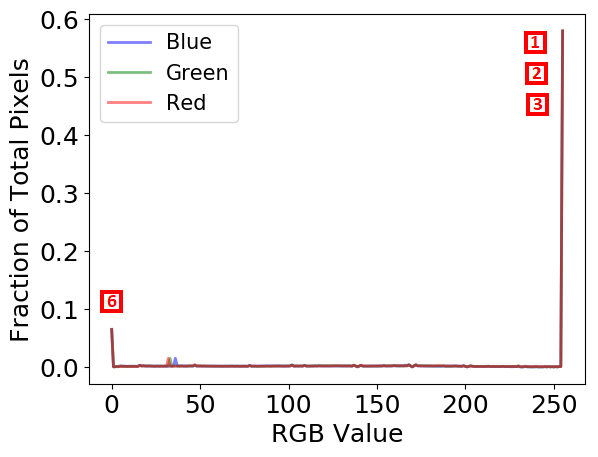
\includegraphics[width=0.58\columnwidth]{./figure/609a_news_light.png}\quad
		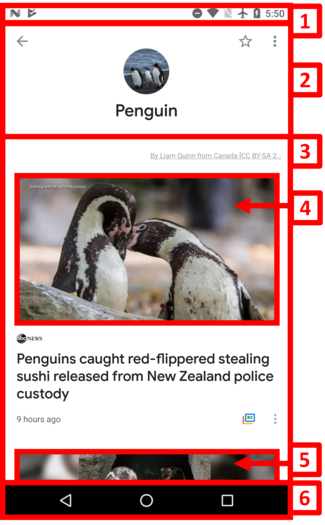
\includegraphics[width=0.27\columnwidth]{./figure/659a_news_light.png}
		\caption{\name output for light mode}
	\end{subfigure}
	\begin{subfigure}[]{\columnwidth}
		\centering
		% \includegraphics[width=0.58\columnwidth]{./figure/608_news_dark.pdf}\quad
		% \frame{\includegraphics[width=0.27\columnwidth]{./figure/658_news_dark.png}}
		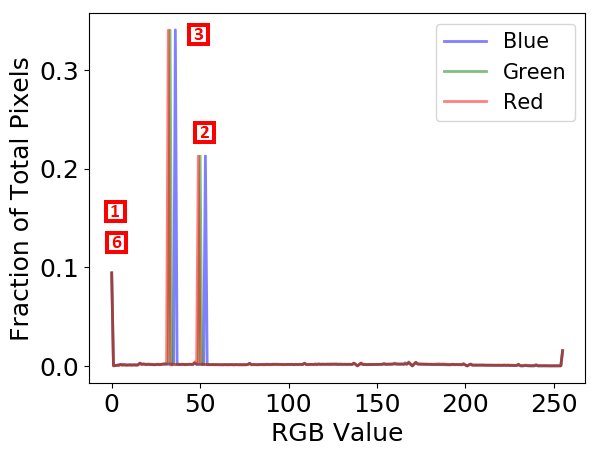
\includegraphics[width=0.58\columnwidth]{./figure/608a_news_dark.png}\quad
		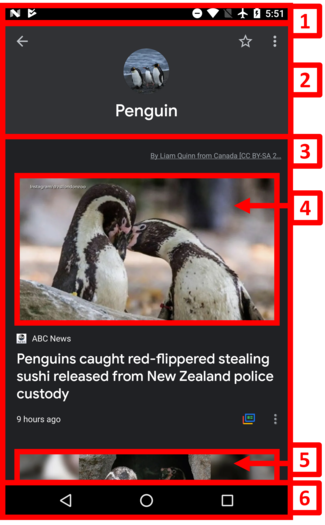
\includegraphics[width=0.27\columnwidth]{./figure/658a_news_dark.png}
		\caption{\name output for dark mode}
	\end{subfigure}
	% \\
	\begin{subfigure}[]{\columnwidth}
	\begin{subfigure}[]{0.42\columnwidth}
		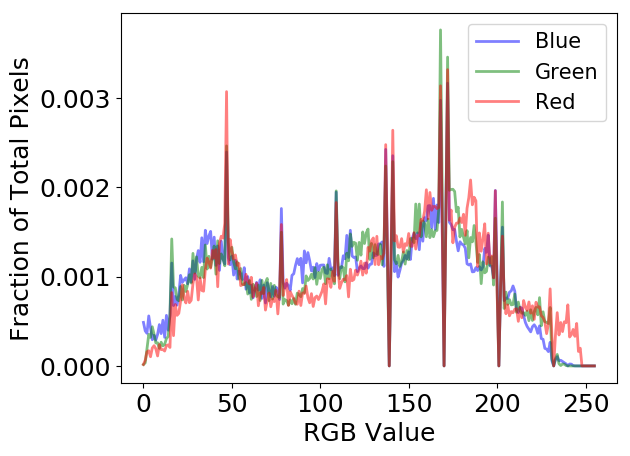
\includegraphics[width=\columnwidth]{./figure/692a_news_penguin.png}
		\caption{Pixel color histogram of the penguin image.}
		\label{fig:case_study_embedde_object}
	\end{subfigure}
	\begin{subfigure}[]{0.38\columnwidth}
	\centering
	{ \scriptsize
	\begin{tabular}{ | l | r | r | r | }
		\hline
		     & \multicolumn{3}{|c|}{Power Reduction (mA)}\\
		\cline{2-4}
                Part & Pixel 2 & Moto Z3 & Pixel 4 \\
		\hline
		1 &   9  &  12 &   11  \\
		2 &  64  &  86 &   76  \\
		3 & 100  & 135 &  120  \\
		4 &   0  &   0 &    0  \\
		5 &   0  &   0 &    0  \\
		6 &   0  &   0 &    0  \\
		\hline
		Total   & 173 & 233 & 207  \\
		\hline
	\end{tabular}
	}
	\caption{OLED power saving (from \name per-component output}		
	\end{subfigure}
        \vspace{-0.1in}
	\end{subfigure}
	\caption{Google News: Headlines activity.}
        \vspace{-0.20in}
	\label{fig:case_study_news}
\end{figure}

\if 0
\begin{figure}[th]
	\begin{subfigure}[]{\columnwidth}
		\centering
		% \includegraphics[width=0.58\columnwidth]{./figure/609_news_light.pdf}\quad
		% \frame{\includegraphics[width=0.27\columnwidth]{./figure/659_news_light.png}}
		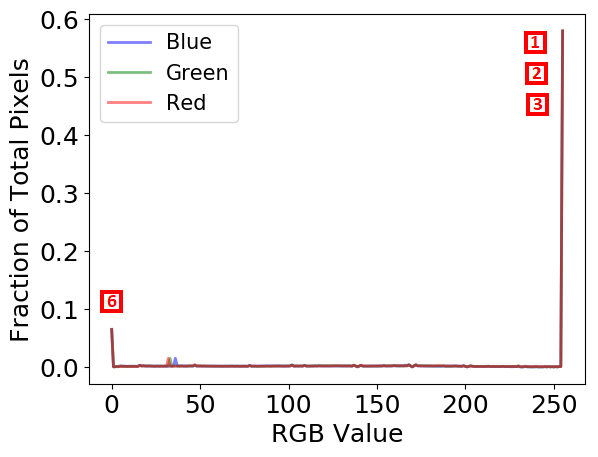
\includegraphics[width=0.58\columnwidth]{./figure/609a_news_light.png}\quad
		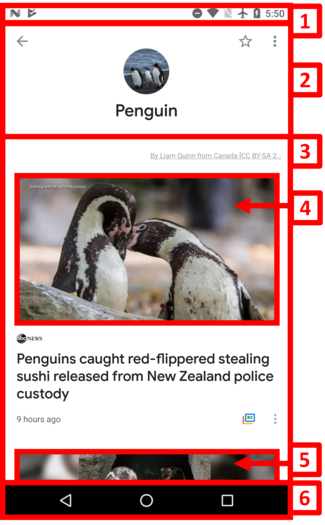
\includegraphics[width=0.27\columnwidth]{./figure/659a_news_light.png}
		\caption{\name output for Light mode}
	\end{subfigure}
	\begin{subfigure}[]{\columnwidth}
		\centering
		% \includegraphics[width=0.58\columnwidth]{./figure/608_news_dark.pdf}\quad
		% \frame{\includegraphics[width=0.27\columnwidth]{./figure/658_news_dark.png}}
		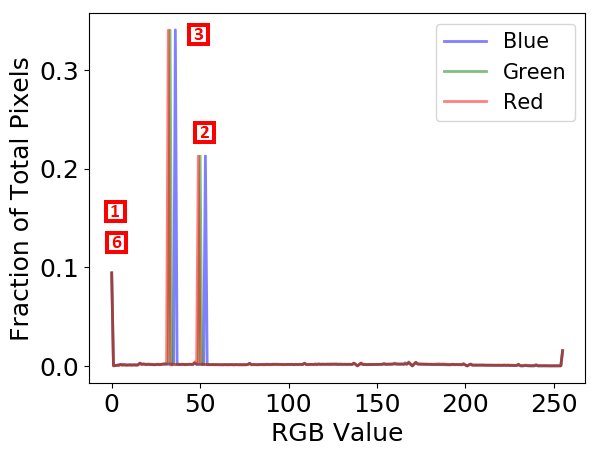
\includegraphics[width=0.58\columnwidth]{./figure/608a_news_dark.png}\quad
		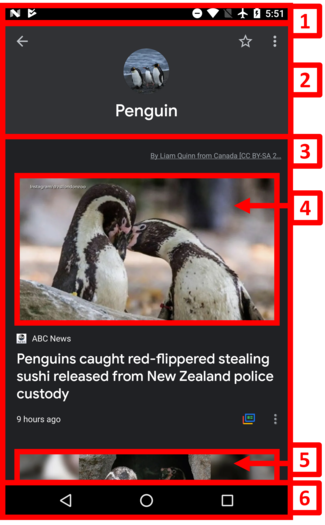
\includegraphics[width=0.27\columnwidth]{./figure/658a_news_dark.png}
		\caption{\name for Dark mode}
	\end{subfigure}
	\\
	\begin{subfigure}[]{\columnwidth}
	\centering
	{ \small
	\begin{tabular}{ | l | r | r | r | }
		\hline
		     & \multicolumn{3}{|c|}{Power Reduction (mA)}\\
		\cline{2-4}
                Part & Nexus 6 & Pixel 2 & Moto Z3 \\
		\hline
		1 &   6  &   8 &   10  \\
		2 &  46  &  59 &   77  \\
		3 &  78  &  97 &  129  \\
		4 &   0  &   0 &    0  \\
		5 &   0  &   0 &    0  \\
		6 &   0  &   0 &    0  \\
		\hline
		Total   & 130 & 164 & 216  \\
		\hline
	\end{tabular}
	}
	\caption{OLED power saving (from \name per-component output}		
        \vspace{-0.1in}
	\end{subfigure}
	\caption{Google News: Headlines activity.}
        \vspace{-0.20in}
	\label{fig:case_study_news}
\end{figure}

\fi
\input activities.tex
